\subsection{女权 or 女拳}
\begin{frame}{部分“女权语录”}
    \begin{block}{}
        \begin{center}
            
\includegraphics[width=.85\textwidth]{../docs/img/4-7.jpg}
        \end{center}
    \end{block}
\end{frame}

\begin{frame}{女权 or 女拳}
    \begin{center}
        \animategraphics[autoplay, loop, controls, width=.9\textwidth]{10}{../docs/img/meme/magick/1-}{0}{19}
    \end{center}
\end{frame}



\subsection{我们真正追求的女权}
\begin{frame}{什么才是我们真正追求的女权呢?}
    \begin{block}{女权主义}
        指为结束性别主义(sexism)、性剥削(sexual exploitation)、性歧视和性压迫(sexual oppression),促进性阶层平等而创立和发起的社会理论与政治运动,在对社会关系进行批判之外也着重于性别不平等的分析以及推动性底层的权利、利益与议题。
    \end{block}
    \begin{block}{}
        女权就是\textbf{男女平等}而不是女尊男卑,女人可以强,男人可以弱,一个团结的集体,应该是相对强的人保护相对弱一些的人,而不是按照性别粗暴地定义一个人是强者还是弱者。每个人都有选择自己生活的权利,能力出众事业心强的女性,可以正常追求自己的事业而不是被周围的环境逼婚,喜欢照顾家人的家庭煮夫也不会被随意嘲讽没出息。当然权利的平等也意味着义务的平等,不然就成了田园女权了。
    \end{block}
\end{frame}

\begin{frame}{为女权主义正名}
    \begin{block}{}
        在中国,我们应当郑重其事地为女权主义正名,为男女平等的意识形态正名:

        反对我们的政治生活、经济生活、社会生活以及价值观念当中的男性主义;反对对女性这个性别的歧视,努力提高女性在人民代表大会及各级领导班子中所占的比例,提高女性在社会生产劳动中所占的比例,提高女性平均收入水平(目前大约相当于男性平均收入水平的70\%),提高女性在家庭生活中的地位,在整个社会全面实现男女平等的女权主义主张,创造一个女权主义的男女平等的理想社会。
    \end{block}
    \begin{center}
        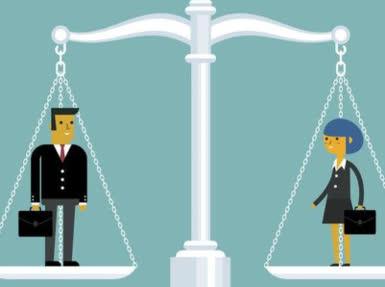
\includegraphics[width=.35\textwidth]{../docs/img/4-6.jpg}
    \end{center}
\end{frame}
